\hypersetup{pdfborder=0 0 0}


%-------------------------------------------------------------------------------------
%\section{Comparison of solitary waves and associated signal from in situ data}
\section[A first evaluation of LES with in-situ \& remote observations]{A first evaluation of LES with in-situ \& remote observations\footnote{Only a selection of in-situ and remote observations of Gibraltar 2020 campaign is studied in the present section. The treatment of the remaining in-situ observations and the preparation of Gibraltar 2022 campaign is carried out in close association with my Ph-D thesis. In the present manuscript, the objective is to provide an as-rigorous-as-possible work including both development of LES, investigation of LES dynamics and evaluation with dedicated observations.}}
\label{sectionCampagne}

\color{blue}The pertinence and the accuracy of the high-resolution Large Eddy Simulations performed so far crucially need to be evaluated based on in-situ or remote observations of both the regional and fine scales of the real ocean. The observation of the latter is somehow difficult at least when these fine scales are localized in small, transient spots. In turn, LES can then appear as a well-adapted tool to help designing the campaign.\color{black}

\subsection{Field campaign Gibraltar 2020 (an overview)}
The field campaign of in situ measurements Gibraltar 2020 has been carried out by the SHOM \color{blue} during the fall of 2020 \color{black} in the strait of Gibraltar and in western part of the Alboran sea aboard the research and survey ship \textit{L'Atalante}. \color{blue} This campaign and the following Gibraltar 2022 campaign are part of the PrometeVs program and LEFE-GEPETO project\color{black}. On-site measures were taken by ship-based instruments from 8/10/2020 to 20/10/2020. Among those, sampling of the water column at both end of the strait were realized at the eastern end of the strait on the 14th and 15th October, and at its western end on the 16th of October.

Additionally, five moorings were deployed as presented in table \ref{tab_moor}, locations are also indicated in figure (\noparref{fig_moor}.b). Mooring M1 is positioned west of the slope of Camarinal Sill. Mooring M3 is placed in the western deep half of CS whereas M2 is positioned in a shallow area at the center. M4 and M5 are positioned near each other at some distance east of CS. Three of the moorings (M1, M3 and M5) are equipped with CTD sensors and the other two (M2 and M4) with ADCP sensors. Sampling frequencies range from a few tens of seconds to one minute.

\begin{table}[!h]
        \centering
        \begin{tabular}{|c|c|c|c|}
                \hline
                Mooring & type & position(deg minute) & time \\ 
                 \hline
                M1 & hydro & N35 55.264 W005 46.739 & 8/10/2020 15h - 9/11/2020 12h\\
                M2 & couranto & N35 55.761 W005 45.288 & 8/10/2020 5h - 17/10/2020 15h\\
                M3 & hydro & N35 54.719 W005 44.459 & 8/10/2020 13h - 22/10/2020 21h\\
                M4 & couranto & N35 55.870 W005 41.020 & 8/10/2020 7h - 17/10/2020 14h\\
                M5 & hydro & N35 56.229 W005 41.026 & 8/10/2020 9h - 1/11/2020 14h\\
                \hline
        \end{tabular}
        \captionof{table}{type of measures, coordinates and date of deployment for moorings during Gibraltar 2020 field campaign.}
        \label{tab_moor}
        %\end{minipage}
\end{table}
In section \ref{section_obs_moor}, mooring data from M2, M4 and M5 are analyzed for a first observation period covering the ten-day period 8/10 to 18/10, when as indicated in table \ref{tab_moor}, both types of moorings data are available.


\subsection{Insights from \color{blue}LES \color{black} simulations in preparation of Gibraltar 2020}

\color{blue}The numerical simulations presented in section \ref{sectionSim3D} is based on a high-resolution, non-hydrostatic model. Atmospheric flues are neglected as a first step toward realistic, high-resolution Large Eddy Simulation of the region of Gibraltar strait.\color{black}\\ 
 \color{green} J'ai interverti les figures pour qu'elles soient citées dans l'ordre.\color{black}
 
\begin{figure}[!h]
% \centering
 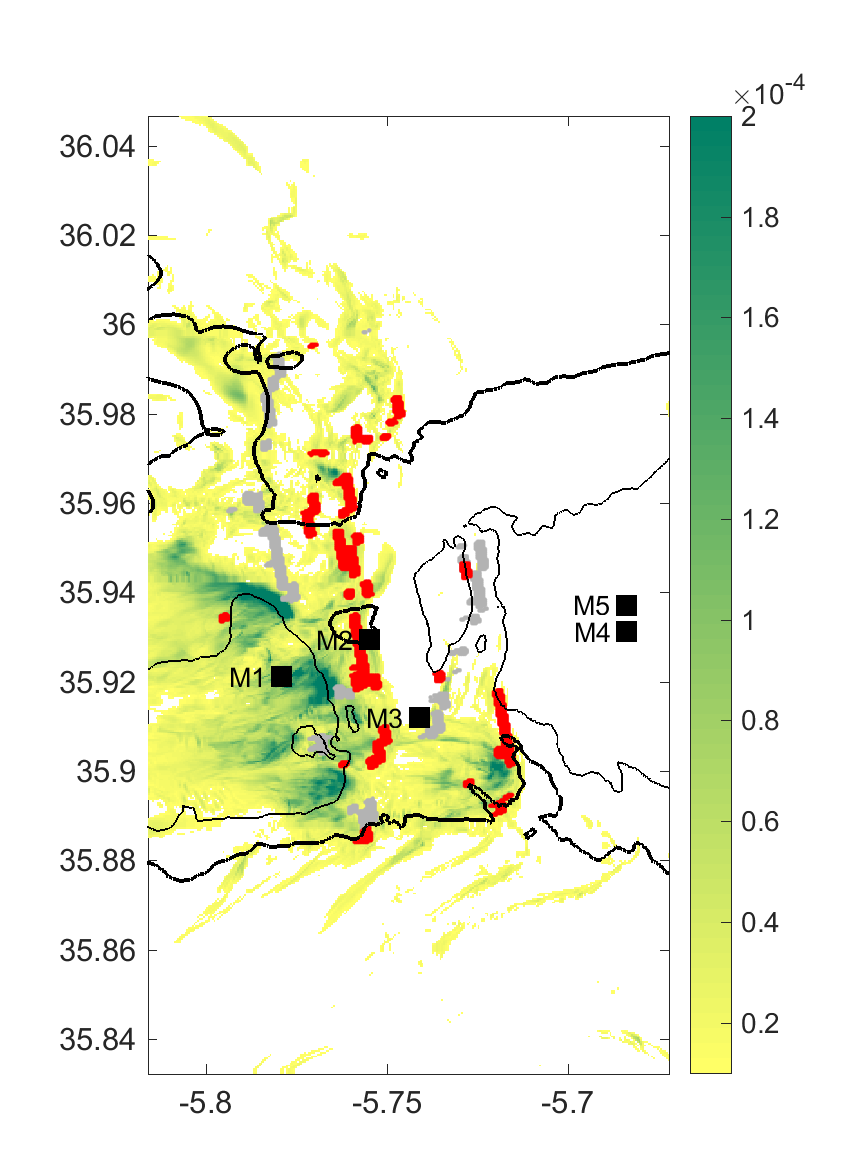
\includegraphics[width=\textwidth]{./GBR3D/Fig_Moor.png}
 \caption {locations of moorings deployed during Gibraltar 2020 (black squares), over the map of standard deviations of parameter Q (colorbar) and the location of the hydraulic jumps of w-type and s-type from high-resolution numerical modelling of the strait of Gubraltar, as presented in section \ref{sectionSim3D}.}
 \label{fig_moor}
\end{figure}
The field of standard deviation of parameter Q and the localization of the hydraulic jumps in figure (\noparref{fig_moor}.b) are for instance issued from those simulations. In combination with external restrictions such as the dense maritime traffic, strong currents and steep slopes of the area, such diagnosis and others were studied to chose the mooring deployment as well as the transect plans (not shown). As an example, M1 was positioned down the western slope of the sill, i.e. downflow of a potential primary instability generation area (see section \ref{PartDiag3D} and \ref{section3DResFlow} for a discussion of this diagnosis in high-resolution numerical simulation).
Figure \ref{fig_SARIES} features a comparison between a SAR image of the strait of Gibraltar with the surface signature of a propagating ISW between CS and the longitude of Tarifa, and the corresponding field of norm of the gradient of surface currents in SimIT showing a traveling wave in the neighborhood. Whereas the shape of the train itself differs in the model and observed fields, the simulation gives an accurate idea of the propagation speed of ISWs in the strait of Gibraltar. This was used to predict position of ISW in relation to the tidal cycle predicted by harmonic prediction (not shown). It was accurate at least in the strait of Gibraltar itself. In the Alboran Sea, where the influence of the gyre on the form of the wave packet is important, prediction was not as accurate. 
Beyond the propagation speed, the high resolution of the model means that the shape itself of the train of ISWs is accurate \color{blue}Ne vient-on pas de dire le contraire juste avant pour ce qui est de la forme ? \color{black}. This is used in the following section \ref{section_obs_moor} to help in the interpretation of mooring data from M4 and M5.

\begin{figure}[!h]
% \centering
 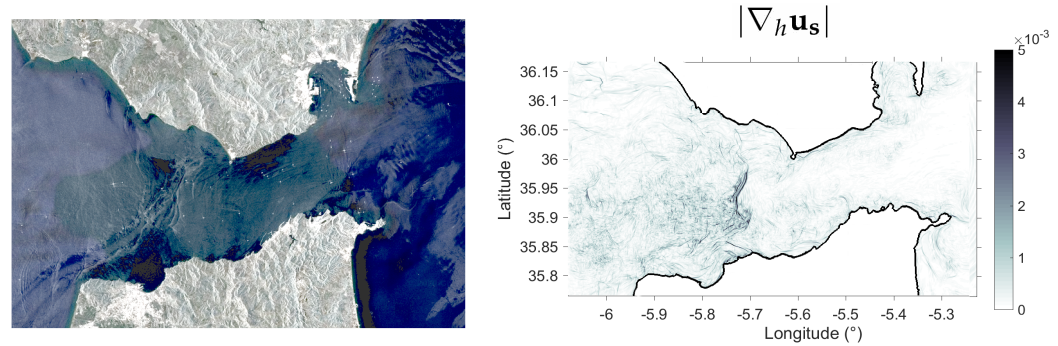
\includegraphics[width=\textwidth]{./GBR3D/Comp_SAR_IES.png}
 \caption {(a) Sentinel-1 Synthetic Aperture Radar (SAR) image (12/09/2017 - 6h18pm UTC). (b) Norm of the gradient of surface horizontal velocity (s-1) in the simulation SimIT (12/09/2017 - 6h30pm or t = 35h30 in simulation time) presented in section \ref{sectionSim3D}.}
 \label{fig_SARIES}
\end{figure}


\subsection{Overview of the mesoscale circulation during the observation period}

The in-situ time period covers one (for ship-based instruments and ADCP moorings) or two (for CTD moorings) neap-spring tide cycles. Figure \noparref{fig_moor_US3}.b shows the depth-averaged zonal component of the current measured at CS (data from M2 mooring). The measures begin during the neap-tide part of the fortnightly cycle. The west Alboran Gyre was also present in the West Alboran Sea during the field campaign (not shown). 

Figure \noparref{fig_moor}.c and d present the $\theta-S$ diagram from ship-based water column sampling. For both figures, each color refers to a different sampling station indicated in figure \noparref{fig_moor}.a.

On the west end of the strait, no Mediterranean water was sampled at the southernmost station and a well-mixed signal could be identified at the northernmost station, delimiting the path of the Mediterranean outflow between 35.7$^{\text{o}}$ and 36$^{\text{o}}$ N. Among the signals of Mediterranean outflow waters, the two most northern stations that reach depths \color{blue} deeper than 400 m show an enhanced mixing with \color{black} NACW.

On the east end of the Strait, WMDW can be found at depth for all stations except the northernmost. For the next two stations south of the latter, as well as the two southernmost stations, WMDW is mixed with intermediate waters. 

The five northernmost stations' surface waters are fresher waters upwelled from the Iberian coast, the intermediate Mediterranean waters sampled at these stations are also warmer and saltier compared to the signal of the remaining four, which is interpreted as LIW.


\subsection{Solitary waves at M4 and M5 mooring and currents at CS at M2 mooring}
\label{section_obs_moor}

\begin{figure}[!h]
% \centering
 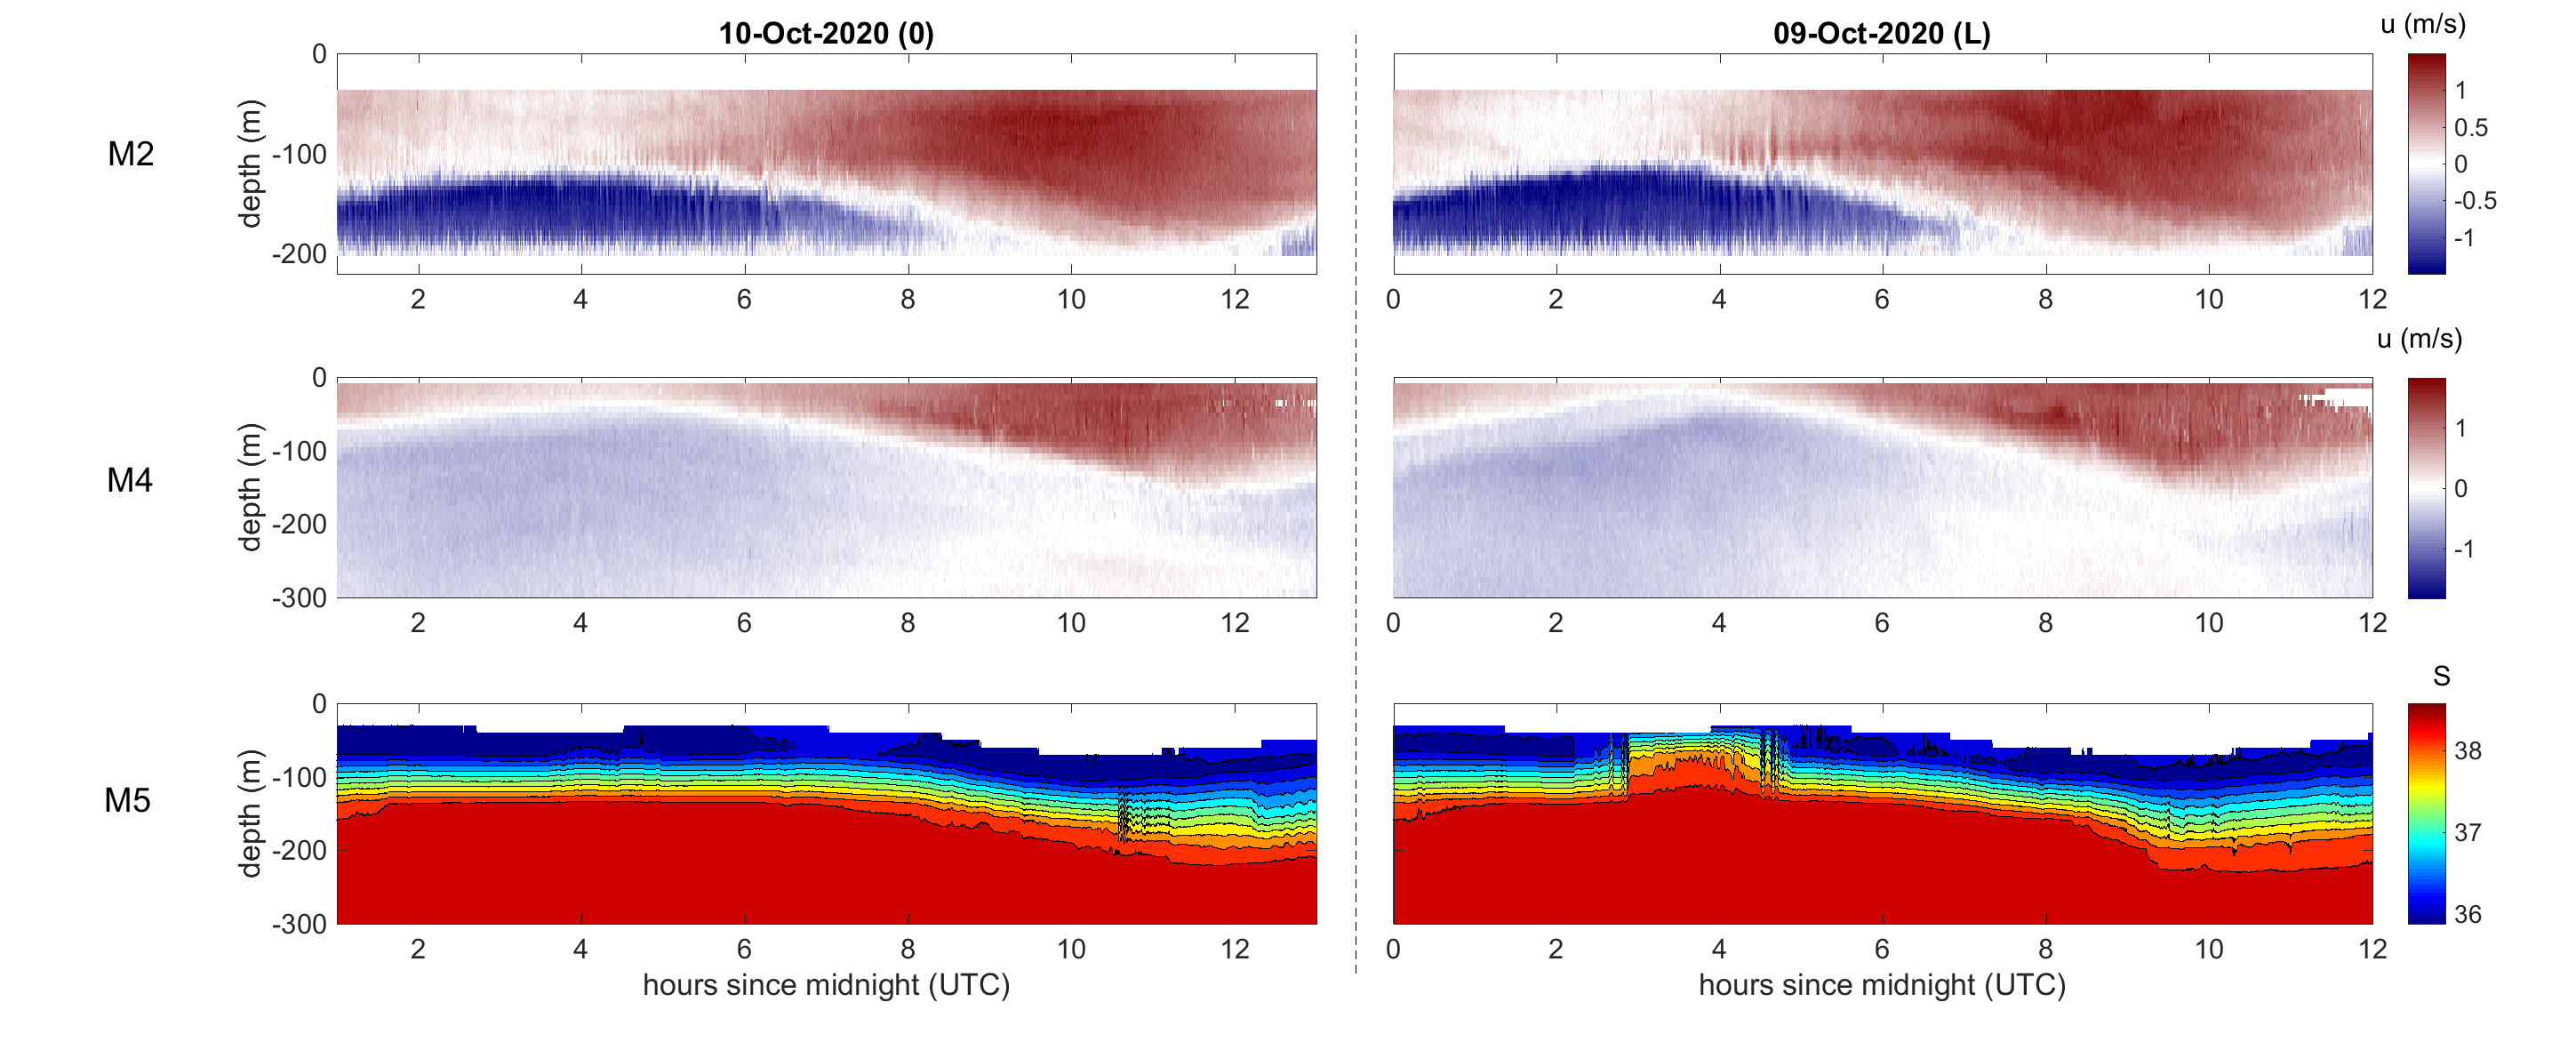
\includegraphics[width=\textwidth]{./GBR3D/US_moorings1.png}
 \caption {timeseries of mooring data over the water column from M2 (upper row), M4 (center row) and M5 (lower row) mooring. The zonal component of currents is represented for M2 and M4 mooring, and the measured salinity at M5 mooring.}
 \label{fig_moor_US1}
\end{figure}

\begin{figure}[!h]
% \centering
 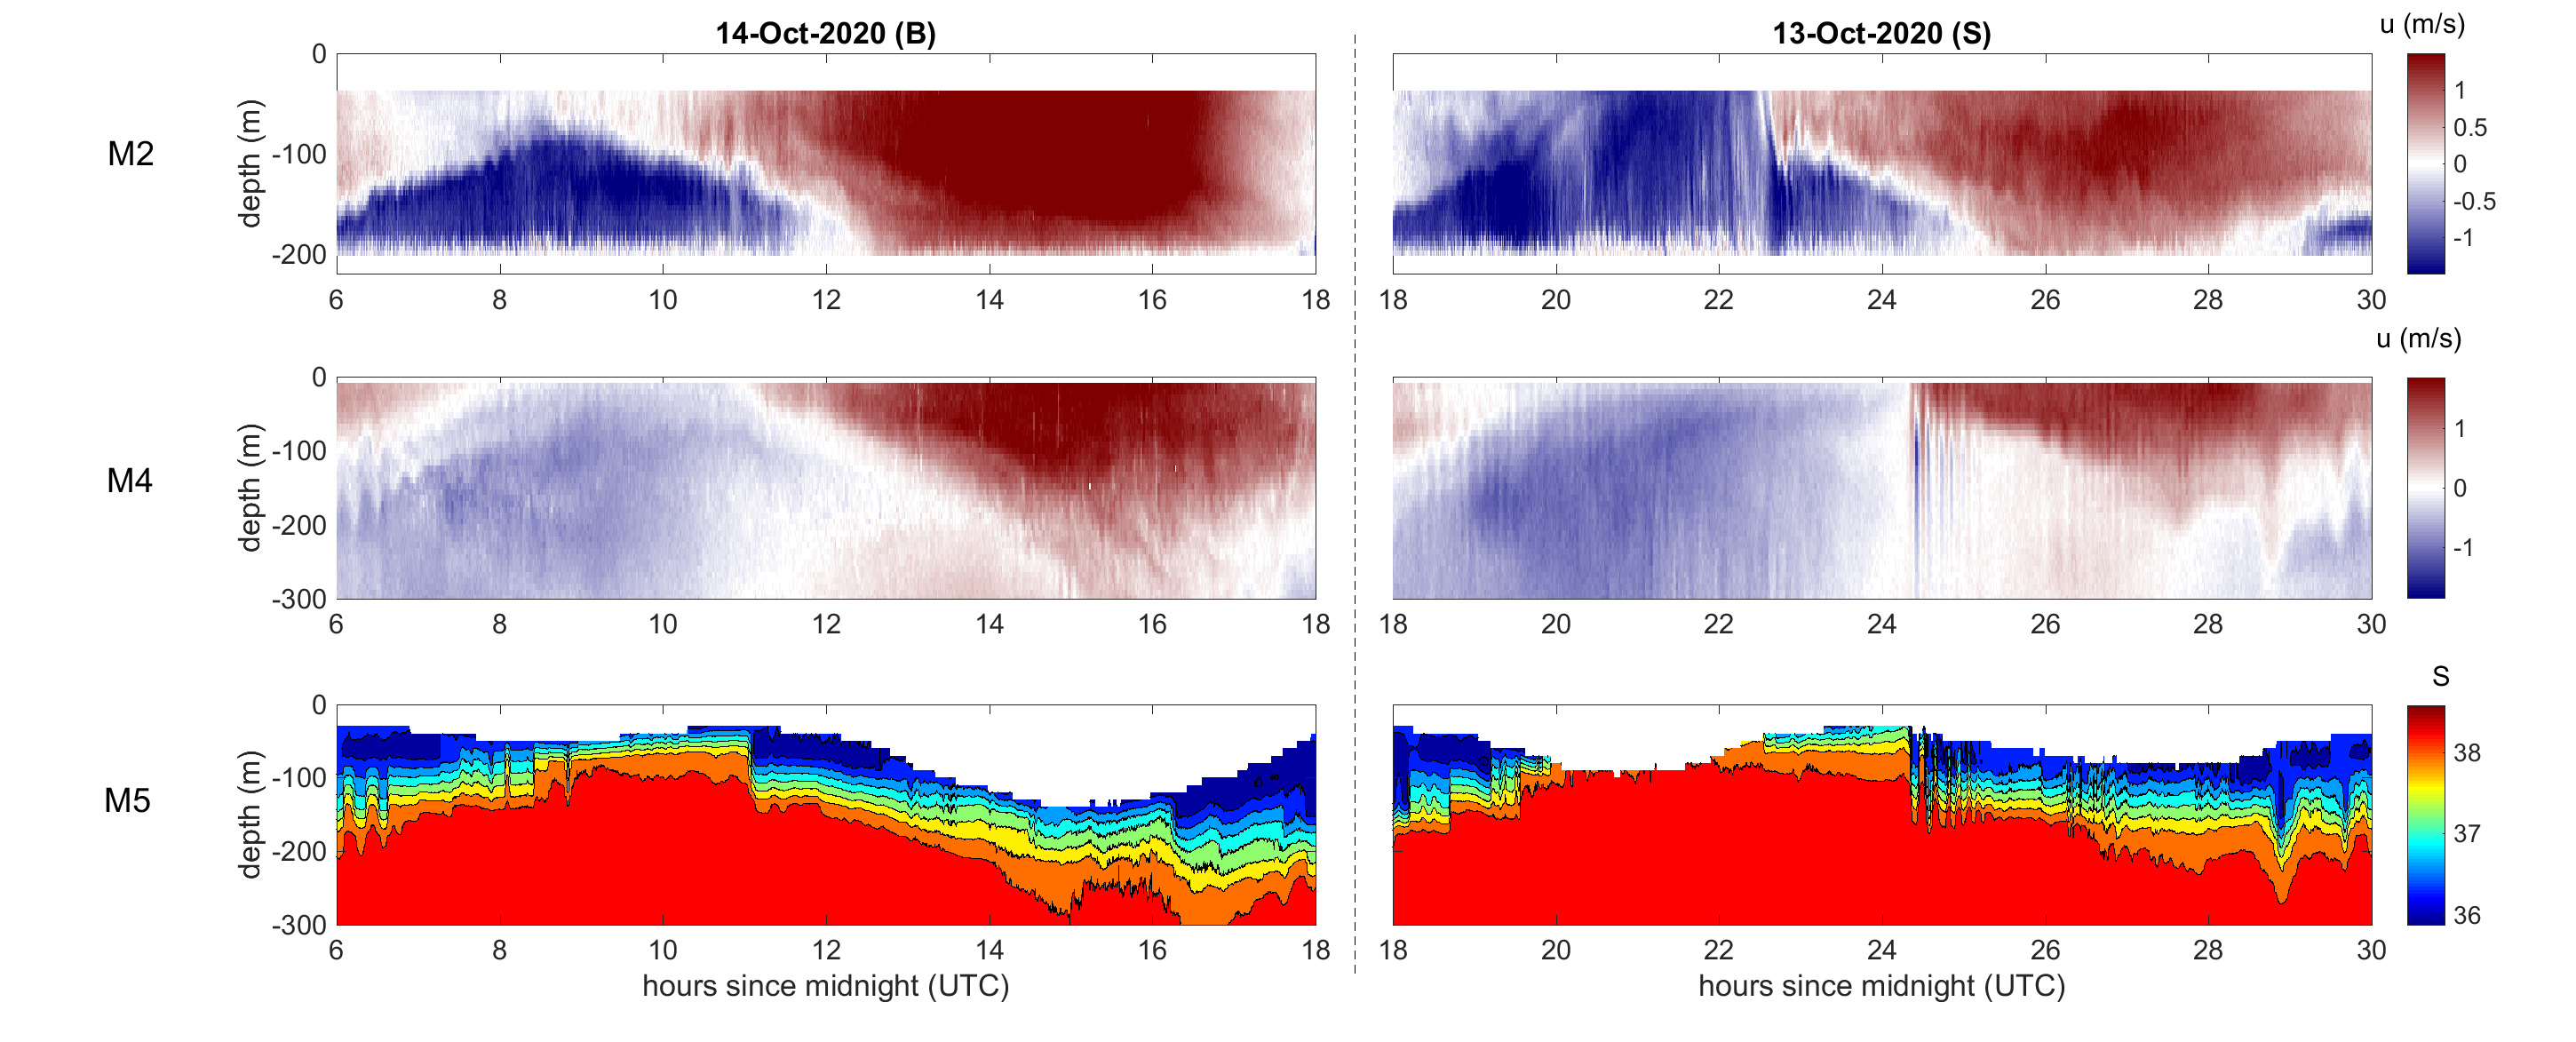
\includegraphics[width=\textwidth]{./GBR3D/US_moorings2.png}
 \caption {same as figure \ref{fig_moor_US1} for a different time-period.}
 \label{fig_moor_US2}
\end{figure}

\begin{figure}[!h]
% \centering
 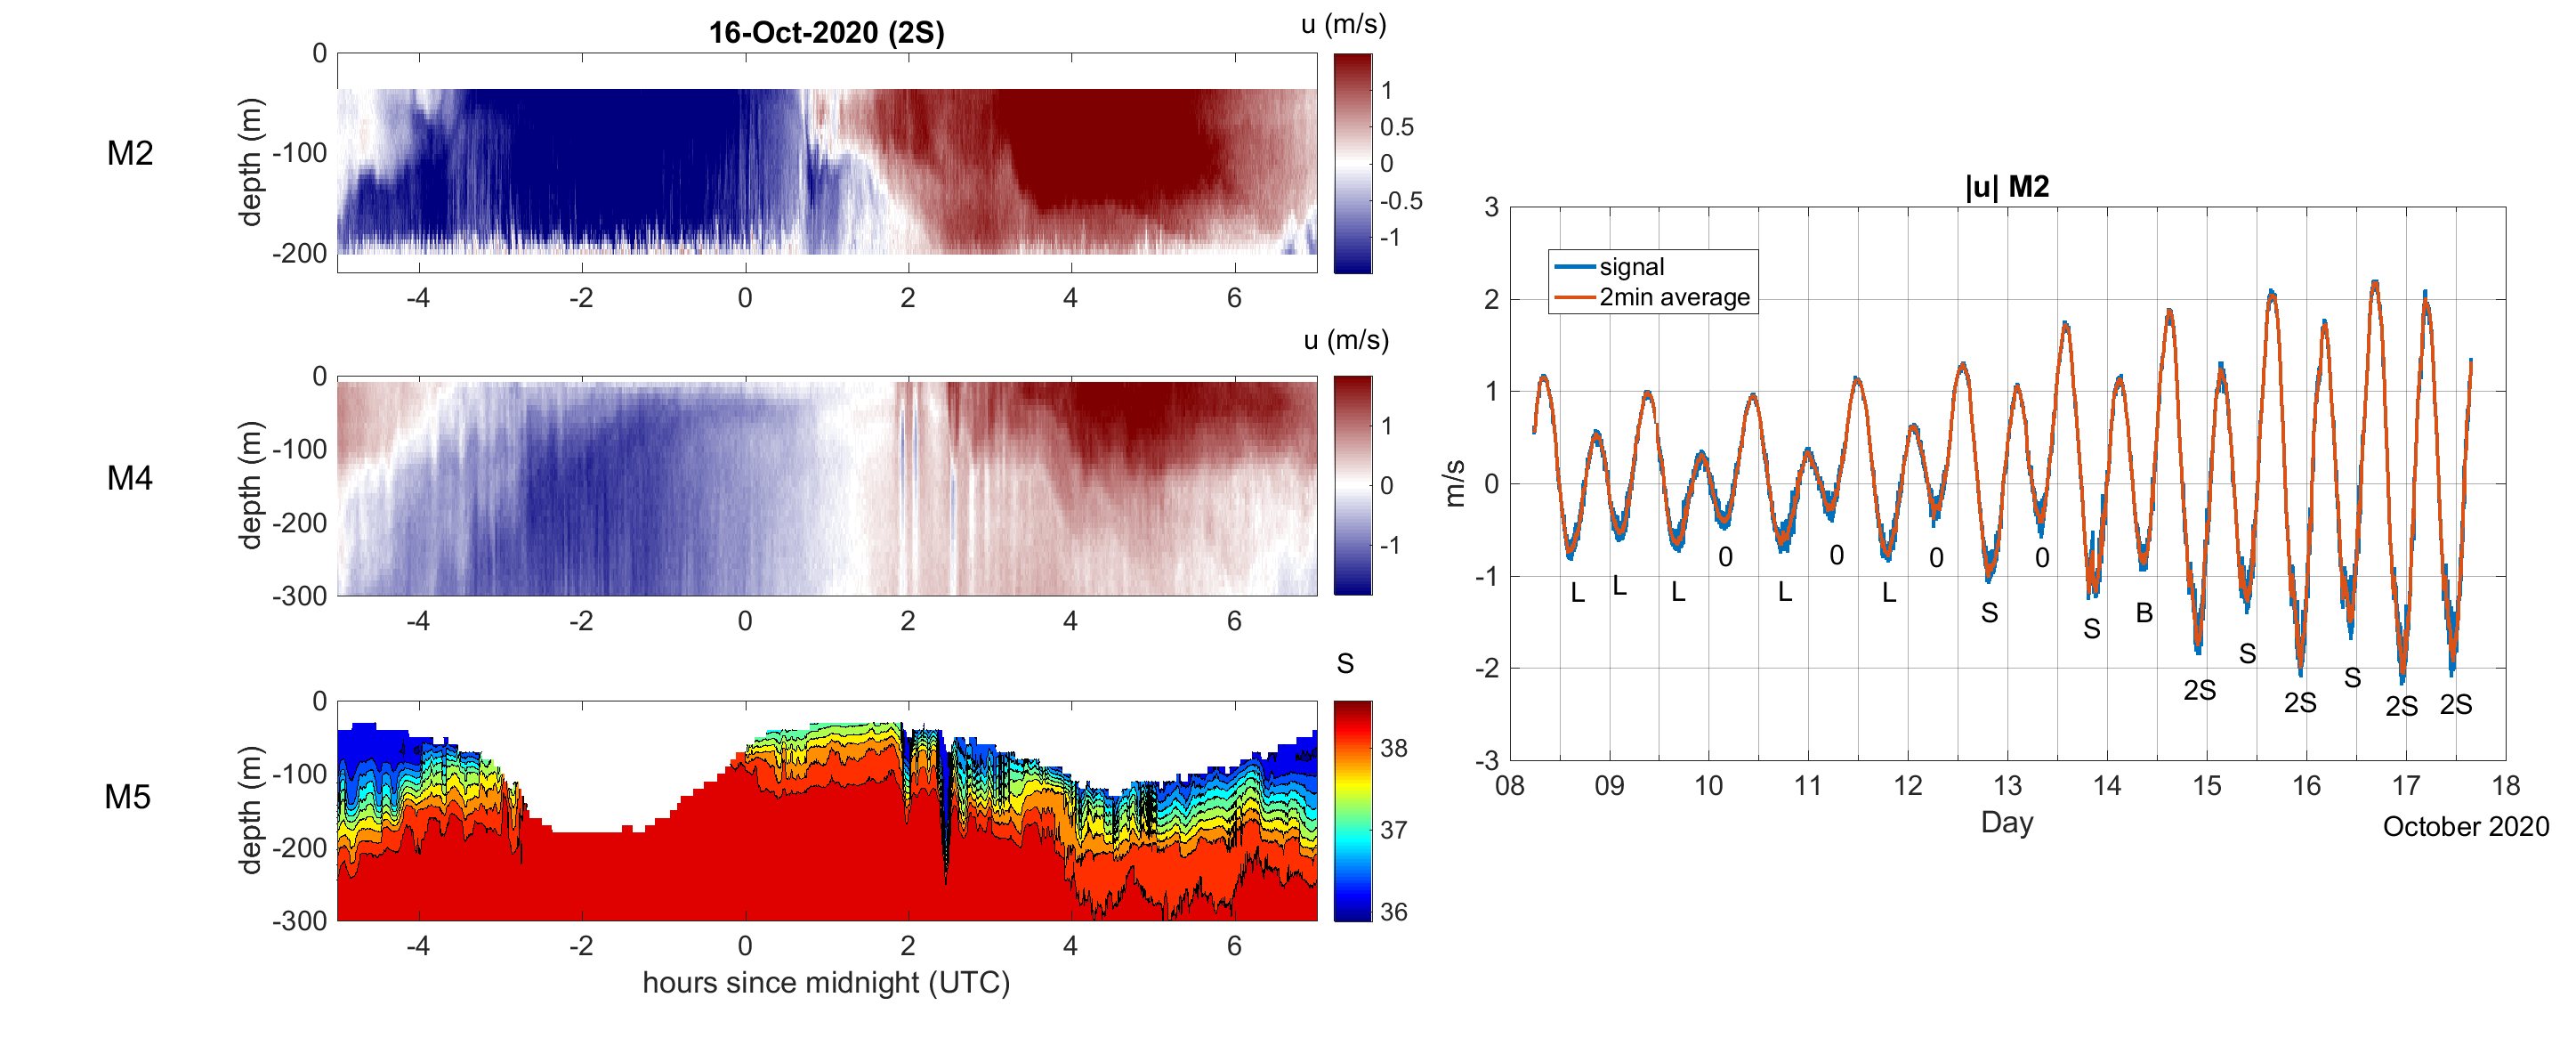
\includegraphics[width=\textwidth]{./GBR3D/US_moorings3.png}
 \caption {(a to c) Same as figure \ref{fig_moor_US1} but for a different time-period. (d) Time-series of depth-averaged signal of the zonal component of currents from M2 data.  \color{blue}For each outflow \color{black} is indicated the type of signal that is observed at M4 and M5 mooring. \color{green}(rajouter SLA tarifa?ou fait trop?) \color{black}}
 \label{fig_moor_US3}
\end{figure}

Figures \ref{fig_moor_US1} to (\noparref{fig_moor_US3}.a) present depth-time records of the zonal velocity (for M2 and M4 mooring) and salinity (for M5 mooring) for five different M2 tidal periods. Note that \color{blue} whereas the whole  \color{black}water column is presented in those figures for the M2 data, only the upper 300 m (of a 500-m-deep water column) are represented here for M4 and M5 data for a better visualization.

Similarly, figure \ref{Fig_moor_USs} presents the zonal velocity and salinity of the upper 300 m of simulated data at a grid point of coordinate  \color{green}() \color{black}, near M4 and M5, from the simulations SimNT (figures \noparref{Fig_moor_USs}a and b), SimIT (c) and SimST (d) of section \ref{sectionSim3D}. Although those simulations cover a different time-period, the data presents similar patterns of internal waves traveling in the water column to the observed data.


\subsubsection{Currents at M2 and M4 mooring}

In the  \color{blue}observations of currents made at mooring M2\color{black}, periods of inflows and outflows can be distinguished respectively as having mostly eastward or westward components over the water column. During inflow periods, there are always at least two hours during which the whole flow measured by the captors is eastward (for example between 10 and 12 hours in figure (\noparref{fig_moor_US1}.a1)). During outflows, the current can be westward at all captors, as is the case in figure (\noparref{fig_moor_US2}.b1) and (\noparref{fig_moor_US3}.a1), but this is not necessarily the case. 

In figures (\noparref{fig_moor_US1}.a1) and (b1), for example, the baroclinic exchange structure of currents is still distinctive during outflows, with a weak eastward flow in the upper 120 m of the water column over a strong westward current. Figure (\noparref{fig_moor_US2}.a1) presents another case for which the flow in the upper water column becomes momentarily weakly westward between t = 7 h and t = 9 h, with a still clear shear interface at 100-m deep.

In the numerical simulations performed in section \ref{sectionSim3D}, an entirely westward flowing water column at M2  \color{blue}mooring \color{black} corresponds to an area of supercritical flow for Atlantic waters when an hydraulic jump is present. This location corresponds to the upflow area of the two types of hydraulic jumps identified in section \ref{sectionSim3D} (s-jump and w-jump), and depicted respectively as grey and black points in figure \ref{fig_moor}.

%Those three cases of sheared currents at M2 during outflows happen in the neap-tide part of the forthnight cycle.

At mooring M4, the flow of the water column can become unidirectional during both outflow and inflow periods during the spring tide part of the fortnightly cycle. In this occasions, a shear area still subsists that matches with the salinity interface between Mediterranean and Atlantic waters identified at mooring M5 (see for example at t = 14 h in figure (\noparref{fig_moor_US2}.a2) and (a3) at depth ranging between 150 and 200 m).

\subsubsection{Propagation of high frequency waves}

\begin{figure}[!h]
% \centering
 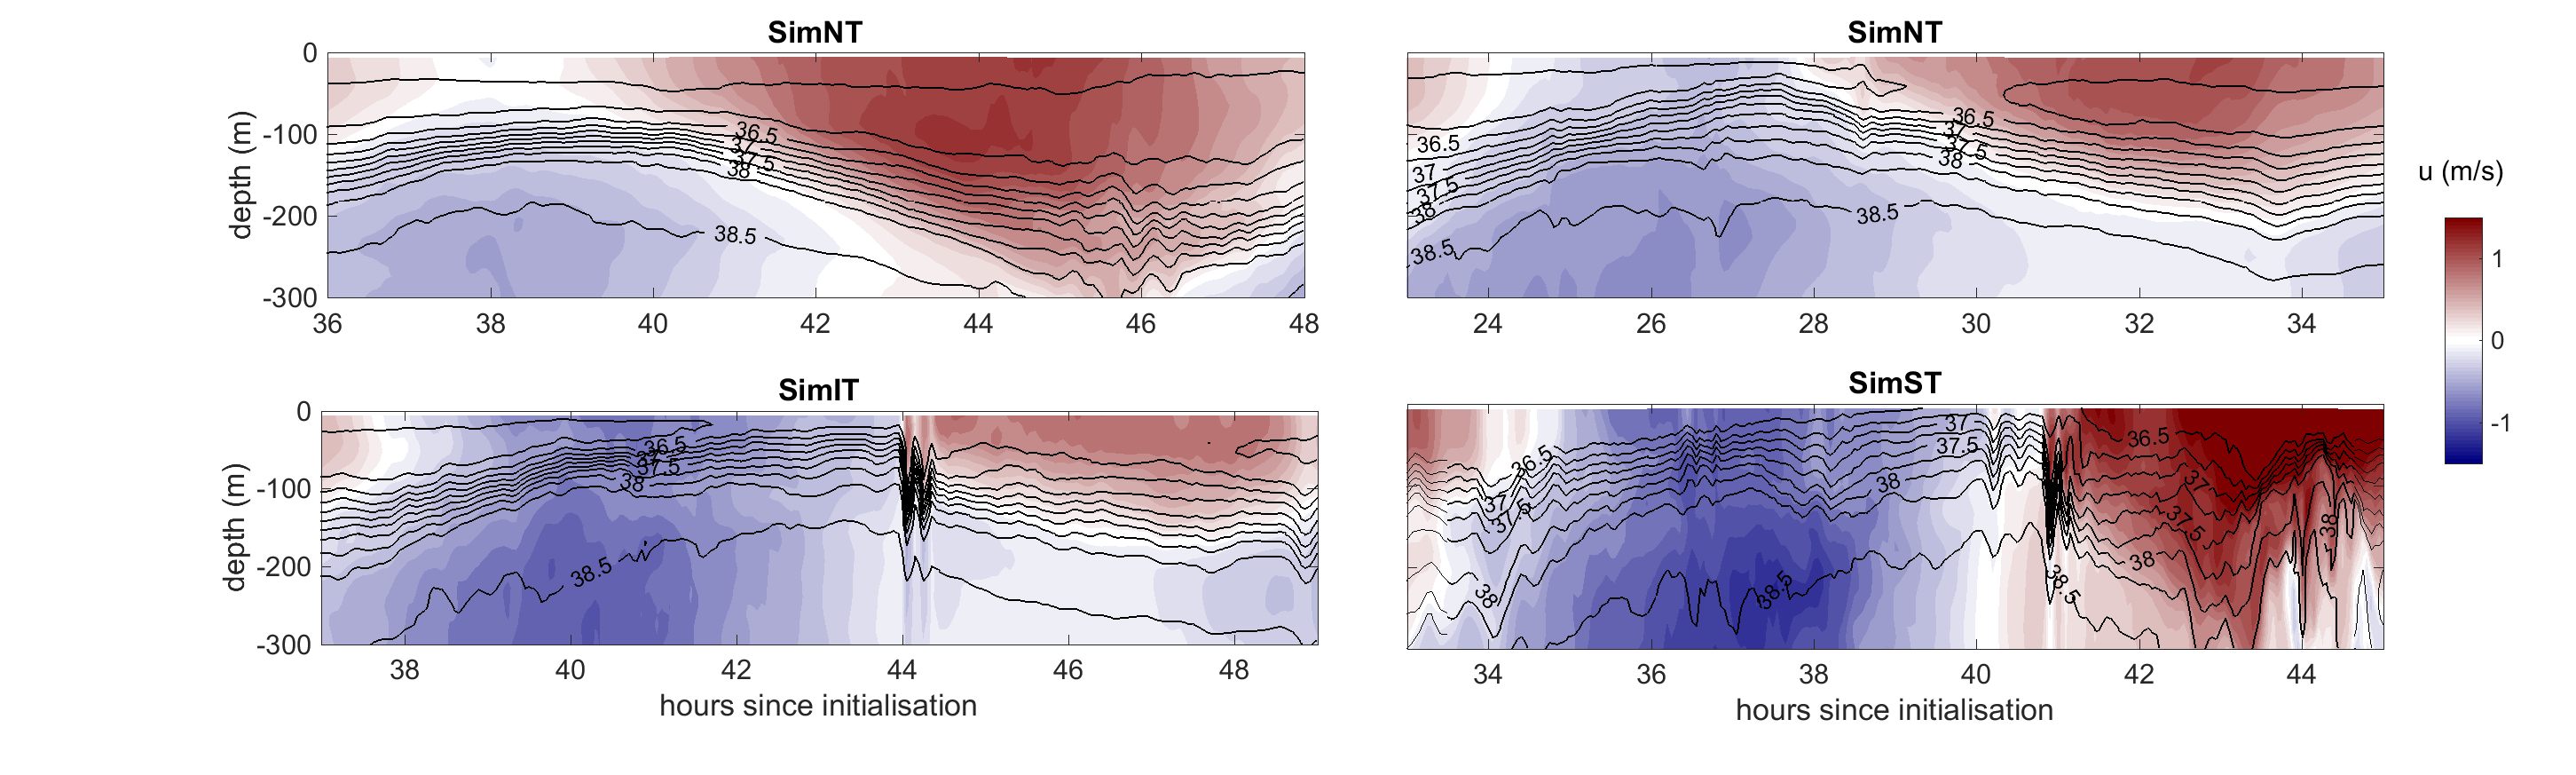
\includegraphics[width=\textwidth]{./GBR3D/US_M4SimMIV.png}
 \caption {time series of salinity (black lines) and zonal velocity (colorbar)  \color{green}in the upper ... m in simulations ... Abscises is simulation time. Mettre des fleches? \color{black}}
 \label{Fig_moor_USs}
\end{figure}

It is on the salinity interface observed at M5 mooring that the signal of propagating internal gravity waves can be spotted, sometimes matching with anomalies in the current field of mooring M4.

Figures (\noparref{fig_moor_US1}.b3) at t = 3 h, (\noparref{fig_moor_US2}.a3) at t = 8h30, and (\noparref{fig_moor_US2}.b3) at t = 19h30, show as a recurring feature an abrupt lifting of the interface, that does not appear in the simulations data of figure \ref{Fig_moor_USs}.

Another recurring signal in M5-mooring data are the large amplitude troughs that can be seen during the inflow period of the tidal cycle. In this data set, it appears clearly in observation data made at t = 29 h in figure (\noparref{fig_moor_US2}.b3). In simulation data (for example t = 49 h in figure (\noparref{Fig_moor_USs}.c)), this signal corresponds to a westward traveling train of ISWs that is generated by reflection of the well-known eastward traveling internal-wave train that is generated at CS.

The focus is now made on the signal showing up at M4 and M5 mooring, usually 3 hours or sooner after the maximal outflow at M2 mooring. Five distinctive types of signals are identified and categorized with letters o, L, B, S, and 2S:\\ 
\color{green} Il faut certainement revoir le système de notation des figures a1, a2, a3, b1... et les indiquer sur les figures correspondantes, je ne m'y retrouve pas trop... \color{black}

\begin{itemize}
\item \underline{Linear-internal tide (o), figures (\noparref{fig_moor_US1}.a2-a3)}: the depth of the interface of salinity at M5 mooring and maximum shear at M4 mooring evolves linearly, except for some low amplitude traveling waves at the interface in M5 mooring at t = 10h30. At M2 mooring (figure \noparref{fig_moor_US1}.a1), there is a distinctive shear in the water column during the preceding outflow, with slightly positive velocity in the upper layer. This signal is also seen in SimNT as shown in figure (\noparref{Fig_moor_USs}.a).
%
\item \underline{Small-amplitude internal wave (L), figures (\noparref{fig_moor_US1}.b2-b3)}: in the salinity data, there is a signal that looks like two internal waves of relatively small amplitude (10 m) at M5 mooring at t = 4h30. At M4 mooring, the depth of maximum shear of zonal velocity still evolves in a linear manner as in the previous (o) case. At M2 mooring (figure \noparref{fig_moor_US1}.b1), the interface of westward flow evolves at the same depth as in the (o) case but in the above layer velocity becomes almost nil from t = 1 h to t = 3h30. This signal is also seen in SimNT in figure (\noparref{Fig_moor_USs}.b) at t = 28.5 h of simulation, and is associated there in the velocity field with a mode-1 anomaly.
%
\item \underline{Internal-traveling bore (B), figures (\noparref{fig_moor_US2}.a2-a3)}: at M5 mooring, the salinity interface drops by 50 m at t = 11 h probably with a westward-propagating internal bore. At M4 mooring, however, the depth of maximum shear still evolves linearly, but \color{blue} before \color{black} the arrival of the internal bore signal, the flow in the water column is negative at all depths. At M2 mooring over CS, the upper layer velocity is nil or lightly negative during the outflow. This type of signal is not recovered in the simulations that have been performed.
%
\item \underline{Train of internal-solitary waves (S), figures (\noparref{fig_moor_US2}.b2-b3)}: a succession of 7 troughs passes at M5 mooring starting at t = 24h15. The first one has an amplitude of 80 m. At M4 mooring, this series corresponds to mode-1 anomalies of the velocity field. At M2 mooring, the flow throughout the water column is westward, with an abrupt return to a sheared two-layer state at t = 22h30, corresponding to the loss of hydraulic control and the release of the western hydraulic jump over CS. In simulations, this type of signal is seen for instance in simIT and presented in figure (\noparref{Fig_moor_USs}.c) with two troughs at  t = 44 h. In these simulations, this type of signal at mooring M4 and M5 follows the release of a s-jump type of hydraulic jump (i.e., at maximum outflow, the western hydraulic jump is located over the shallowest part of CS).
%
\item \underline{Two close trains of internal-solitary waves (2S), figures (\noparref{fig_moor_US3}.a1-a2)}: five troughs can be seen propagating at M5 mooring starting at t = 2 h. The first one has an amplitude of 80 m and is followed by two short-wavelength, small-amplitude troughs. Then at t = 2h30, an over-100-m amplitude trough propagates at M5 mooring. It is in turn followed by a smaller-amplitude trough. The mode-1 anomaly of the velocity field is seen clearly at M4 mooring for the first two waves, then the fourth larger amplitude one. At M2 mooring, as in the previous (S) case, the flow through the water column transitions from wholly westward to sheared two-layer at t = 1 h. In numerical simulation SimST (figure \noparref{Fig_moor_USs}.d), four waves can be identified. They follow this pattern, \color{blue} the first two waves have decreasing amplitude, the third has a larger amplitude than the first two, and the fourth has a smaller amplitude. \color{black} In this case, this pattern corresponds to two different trains of ISWs.  \color{blue}The first (second) train corresponds to the previously  released hydraulic jump east (west) of CS.\color{black} In the numerical simulations, this signal follows the release of a w-jump (i.e., at maximum outflow the west hydraulic jump is located over the western slope of CS).
\end{itemize}

Both S and 2S signals are linked to westward flow of the whole water column at CS, which should indicate that, as in the numerical simulations, a hydraulic jump was present west of M2 mooring.

\color{blue}The 2S case can be observed in numerical simulations and in figure (\noparref{Fig_moor_USs}.d). \color{black} The amplitude of the first wave which corresponds to the eastern hydraulic jump of CS can be very small. It depends (i) on the northern extent of the eastern hydraulic jump at maximum outflow (i.e., how high a latitude it reaches) and(ii) on the initial angle taken by the released non-linear wave as it first propagates in a slightly southern direction.

As the two sets of ISWs propagate further in the strait, the second train overtakes the first one. Indeed the propagation speed of ISWs depends on the amplitude \color{blue} (the larger the faster) \color{black}, and they merge into a single train of ISWs. Similarly, the "S" structure in simulation appears because the wave released by the western hydraulic jump of CS overtook the eastern one sooner due to their initial closeness.

So although \color{blue} they appear here as being distinct from the S case following an s-jump and from the 2S case following a w-jump in simulations, there might be a possibility \color{black} that slowly propagating waves from an s-jump could also appear as a 2S structure at M4 and M5 mooring.


\subsection{Transition between outflow types \& ISWs generation in Gibraltar strait}

The classification of the previous section is applied to signals at M4 and M5 mooring following each outflow of the first observation period and is marked as annotations in figure (\noparref{fig_moor_US3}.n).

A pattern emerges linking outflow type and strength of the averaged currents at CS. The beginning of the period corresponds to the neap-tide part of the fortnightly cycle, and either (L) or (o) type of outflows are detected, with no hydraulic jump at CS. The first solitary wave is observed at M4 and M5 mooring the 12/10/2020. Due to \color{blue} the diurnal variation \color{black} of the M2 tide, the tidal flow over the following period is weaker (less than 1 m/s) and is an (o) case.

Except for one specific (B) case (14/10/2020), during the remainder of the period, trains of ISWs (with either a S or 2S structure) are propagating through M4 and M5 mooring. The stronger outflows lead to (2S) signals \color{blue} in agreement with the \color{black}numerical simulations presented in section \ref{sectionSim3D}. Under especially strong outflows, the internal hydraulic jump generated over CS is swept downstream as a w-jump, resulting in an initially increased distance between the eastern and western jumps. This distance may not overcome as quickly  \color{blue}when released \color{black} as in the s-jump case. Though as explained previously, for some outflows, the distinction between the S and 2S cases \color{blue} may remain \color{black} subjective.

\color{green}There is a clear threshold over which begin to have , though stratiication conditions are expected to play an importance in it since it would affect supercriticaity condition for the flow. Peux-tu reprendre cette phrase ??? \color{black} In numerical simulations, the transition between \color{blue} periods  \color{black} is expected to be difficult to predict \color{blue} due to its high-sensitivity to bathymetry constraints, to stratification and obviously to tidal forcing.
%sensitivity of the system means it relies on good bathymetric feature of CS to have an accurate strength of the currents, accurate stratification and accurate tidal forcing.

Only one (B) case is observed, it was not featured in numerical simulations so it is less evident whether it can be attributed to the presence of an hydraulic jump over CS. Whereas the variation with depth of currents at M2-mooring site in the preceding outflow shows a shallower interface and more westward currents in the upper layer than for the (o) and (L) cases, it may be more akin to a near supercritical flow regime engendering some form of propagating steepening interfacial disturbance.

It was seen in section \ref{section_sim3D_ISW} that even if no hydraulic jump occurs at CS (at least in numerical simulations), the flow of the barotropic tide in the strait of Gibraltar can lead to a steepening of a long interfacial wave that later develops into a train of ISWs. \color{blue} It is less extensive (extended???) than in the hydraulic jump case, that propagates in the Alboran Sea. \color{black} It then is possible that the mechanism of release of the hydraulic jump may not be the only one responsible for generation of the observed ISWs in the strait of Gibraltar and in the western part of the Alboran Sea.  \color{green}(see \citet{chen_2017} for a summary of various ISW generation mechanisms... (intro + figure 15...point voc)) 

(Ajouter SAR 6h20 9/10?.... See a propagating wave in Alboran, previously only (L) outflows...)\color{black}

\color{blue}
\subsection{Discussion \& perspectives}

A first confrontation between LES and observations has been carried out showing at least a qualitative agreement.  \color{green}Je te laisse compléter en reprenant une ou deux comparaisons que tu penses encourageantes. En particulier le lien avec les structures o, S etc...\\
\color{blue}This confrontation also clearly showed the limits of the modelling strategy used so far. Several improvements have already been made but are still been evaluated and, as a consequence, have not been included in the present section. 
\begin{itemize}
\item Atmospheric fluxes are specified at the surface of the ocean.  This provides a better representation of the stratification in the upper surface and has important consequences on the characteristics of the pycnocline and thus on the characteristics of the internal waves, bores and solitons.
\item The high-resolution dynamics in the strait of Gibraltar is explicitly simulated by downscalling the regional circulation. A three-step embedding has already been carried out using AGRIF library from 900-m to 50-m resolution simulations through a 250-m resolution implementation.
\end{itemize}
 \color{black}
\color{black}

\section{Conclusion}

\color{green} Rappel méthode, bilan développement LES, bilan maquette...\color{black}